\def\template{../template/}
\makeatletter \ifx\input@path\@undefined \def\input@path{{\template}} \else \g@addto@macro\input@path{{\template}} \fi \makeatother


% -- Packages --------------------------------------------------------%
\documentclass{rwth-beamer}
\usepackage{diagbox}
\usepackage{pgfplotstable}

% -- New Commands --------------------------------------------------------%
\newcommand*{\TitleFont}{%
      %\usefont{\encodingdefault}{\rmdefault}{b}{n}%
      \fontsize{13}{16}%
      \selectfont}
      
% -- Title --------------------------------------------------------%
\title[Magnetic Domain-Wall Racetrack Memory]{\TitleFont Racetrack Memory}
\author{Martin Frank}
\institute{MathCCES}
\titlegraphic{
\includegraphics[trim=60pt 95pt 60pt 95pt, clip, height=2em]{\template logo/cammp}}
\date{Voeren, June 5, 2017}
\backgroundgraphic{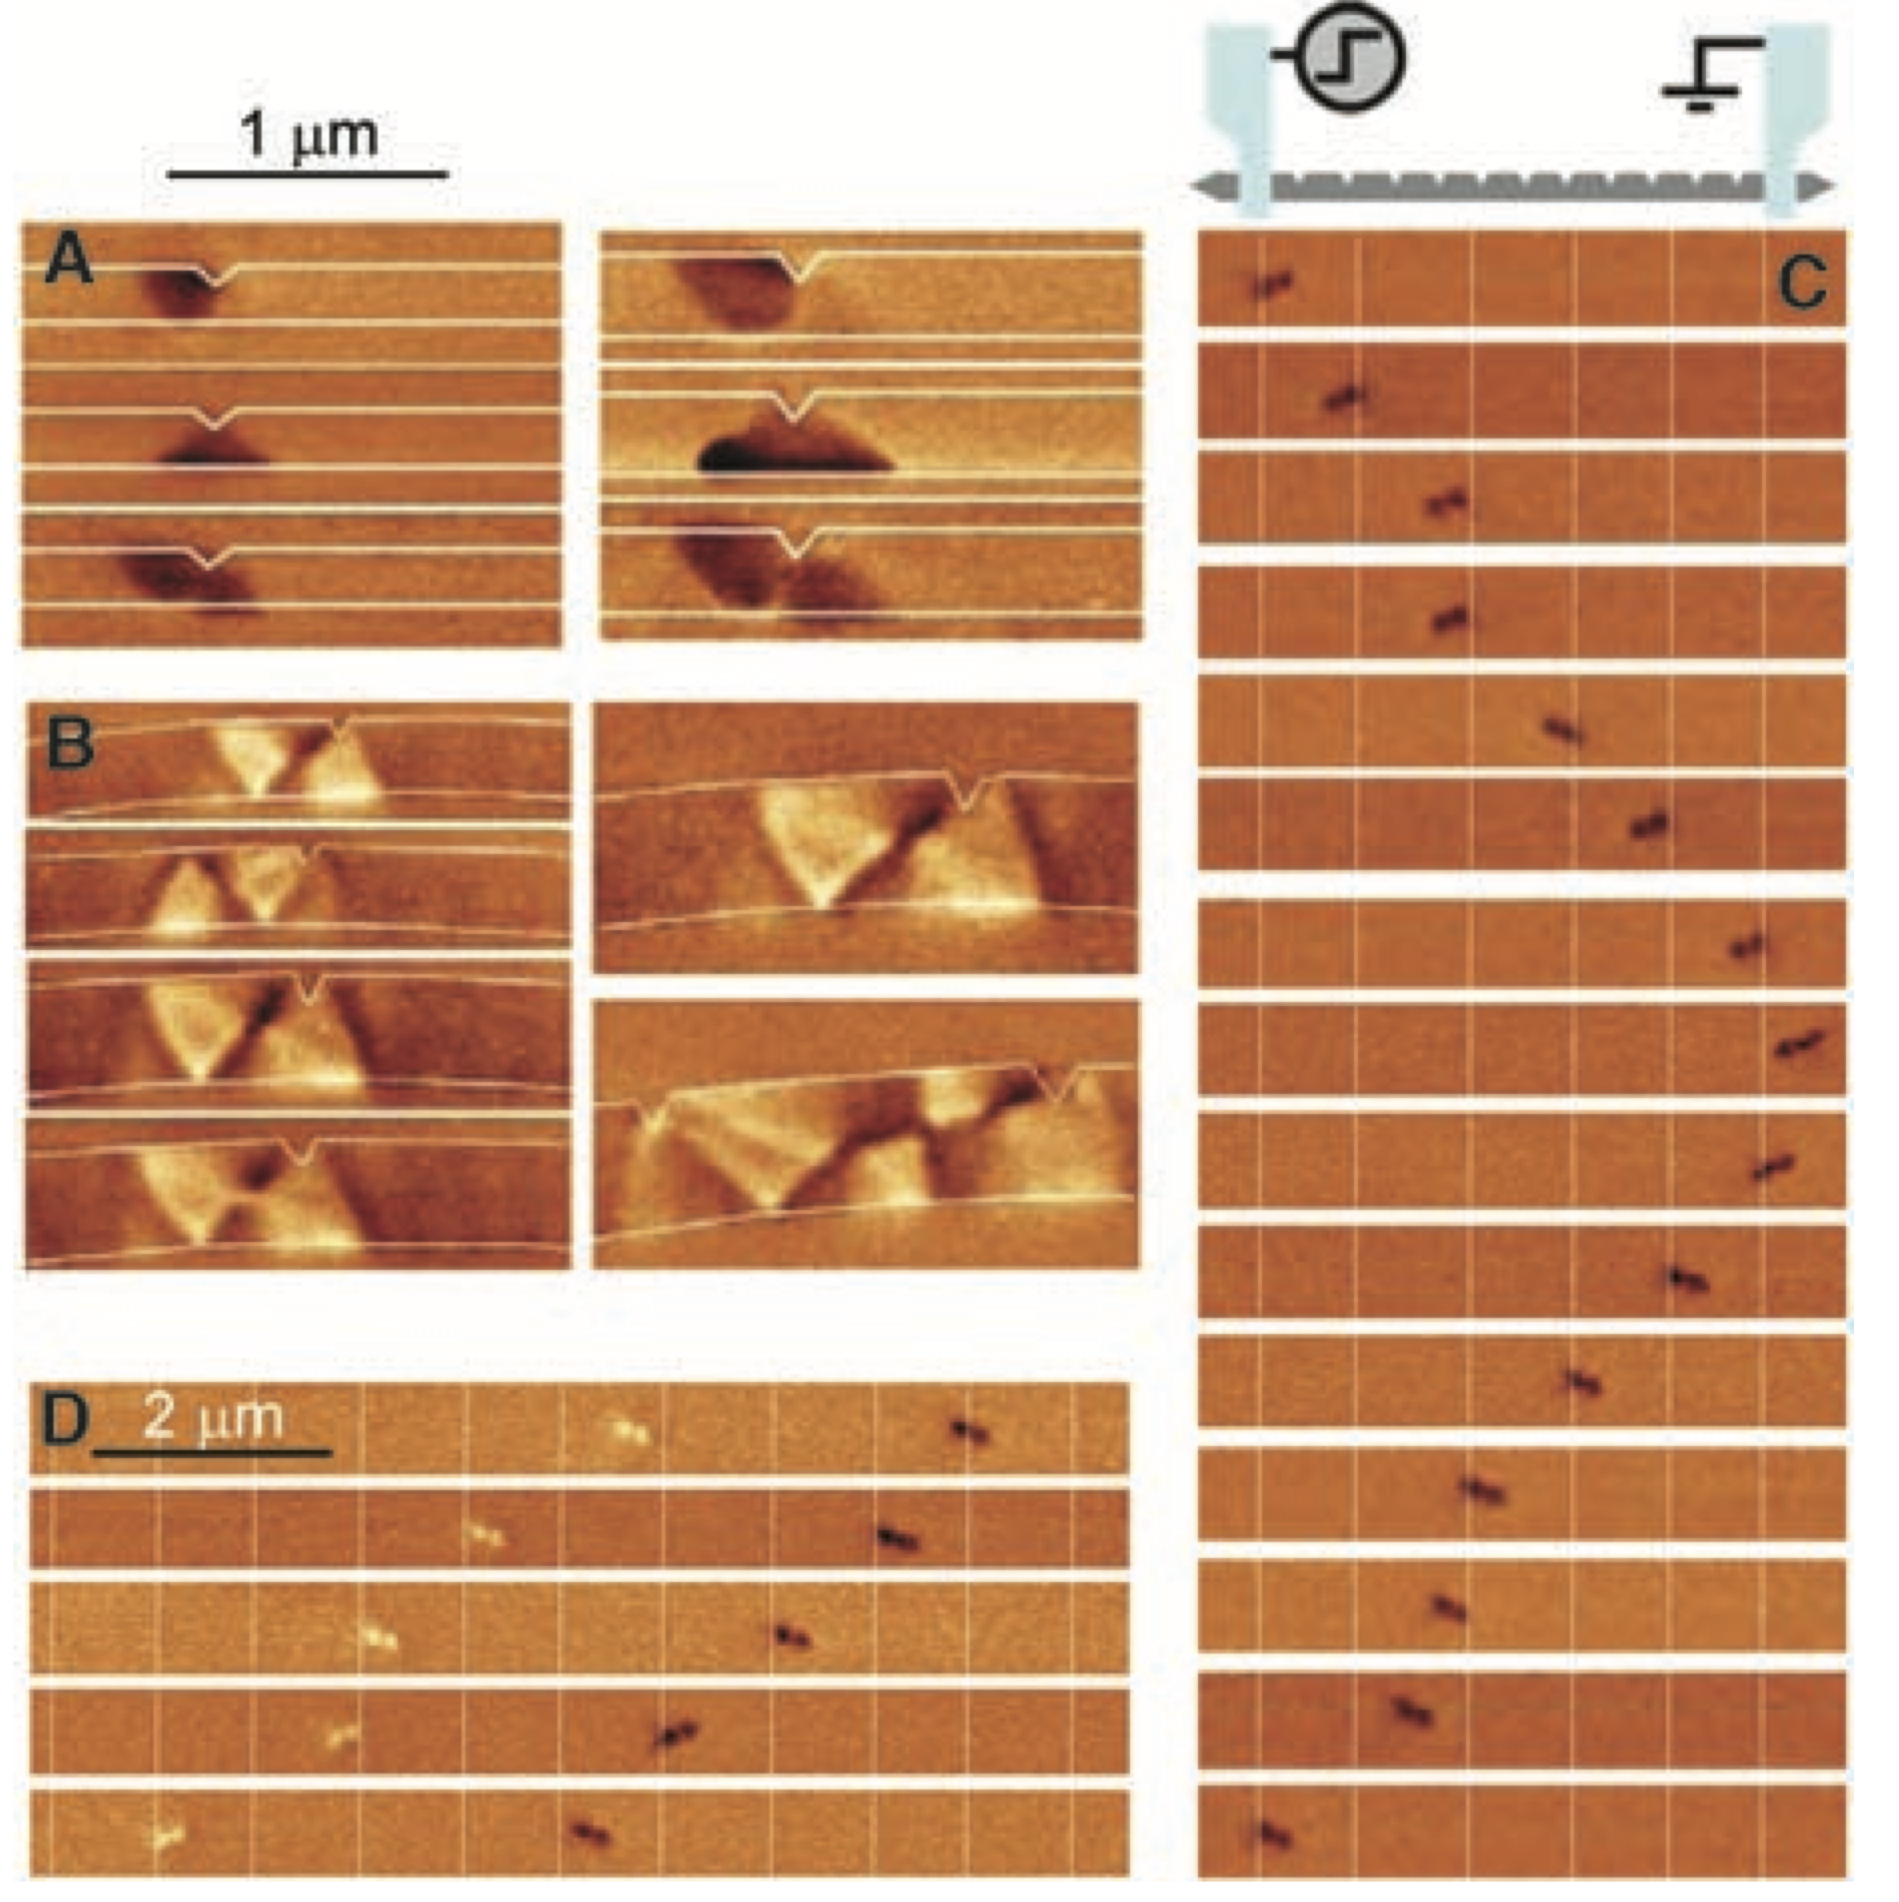
\includegraphics[trim=0pt 0pt 0pt 80pt, clip, width=\paperwidth]{../figs/DomainWalls}}
\footline{\insertauthor\enspace|\enspace\insertshorttitle}



%----------------------------------------------------------%
\begin{document}

	% Title page
	\maketitle

	\begin{frame}[c]
		\frametitle{What is Racetrack Memory?}
		\begin{minipage}{0.7\linewidth} 
		{\bfseries Magnetic domain walls:}
		\begin{itemize}
			\item Formed at the boundaries between magnetic domains
			\item Magnetized in opposite directions (up or down)
		\end{itemize}
		{\bfseries Racetracks:}
		\begin{itemize}
			\item Ferromagnetic nanowire
			\item Data encoded as a pattern of magnetic domains along a portion of the wire
		\end{itemize}
		\end{minipage}\hfill
		\begin{minipage}{0.3\linewidth} 
		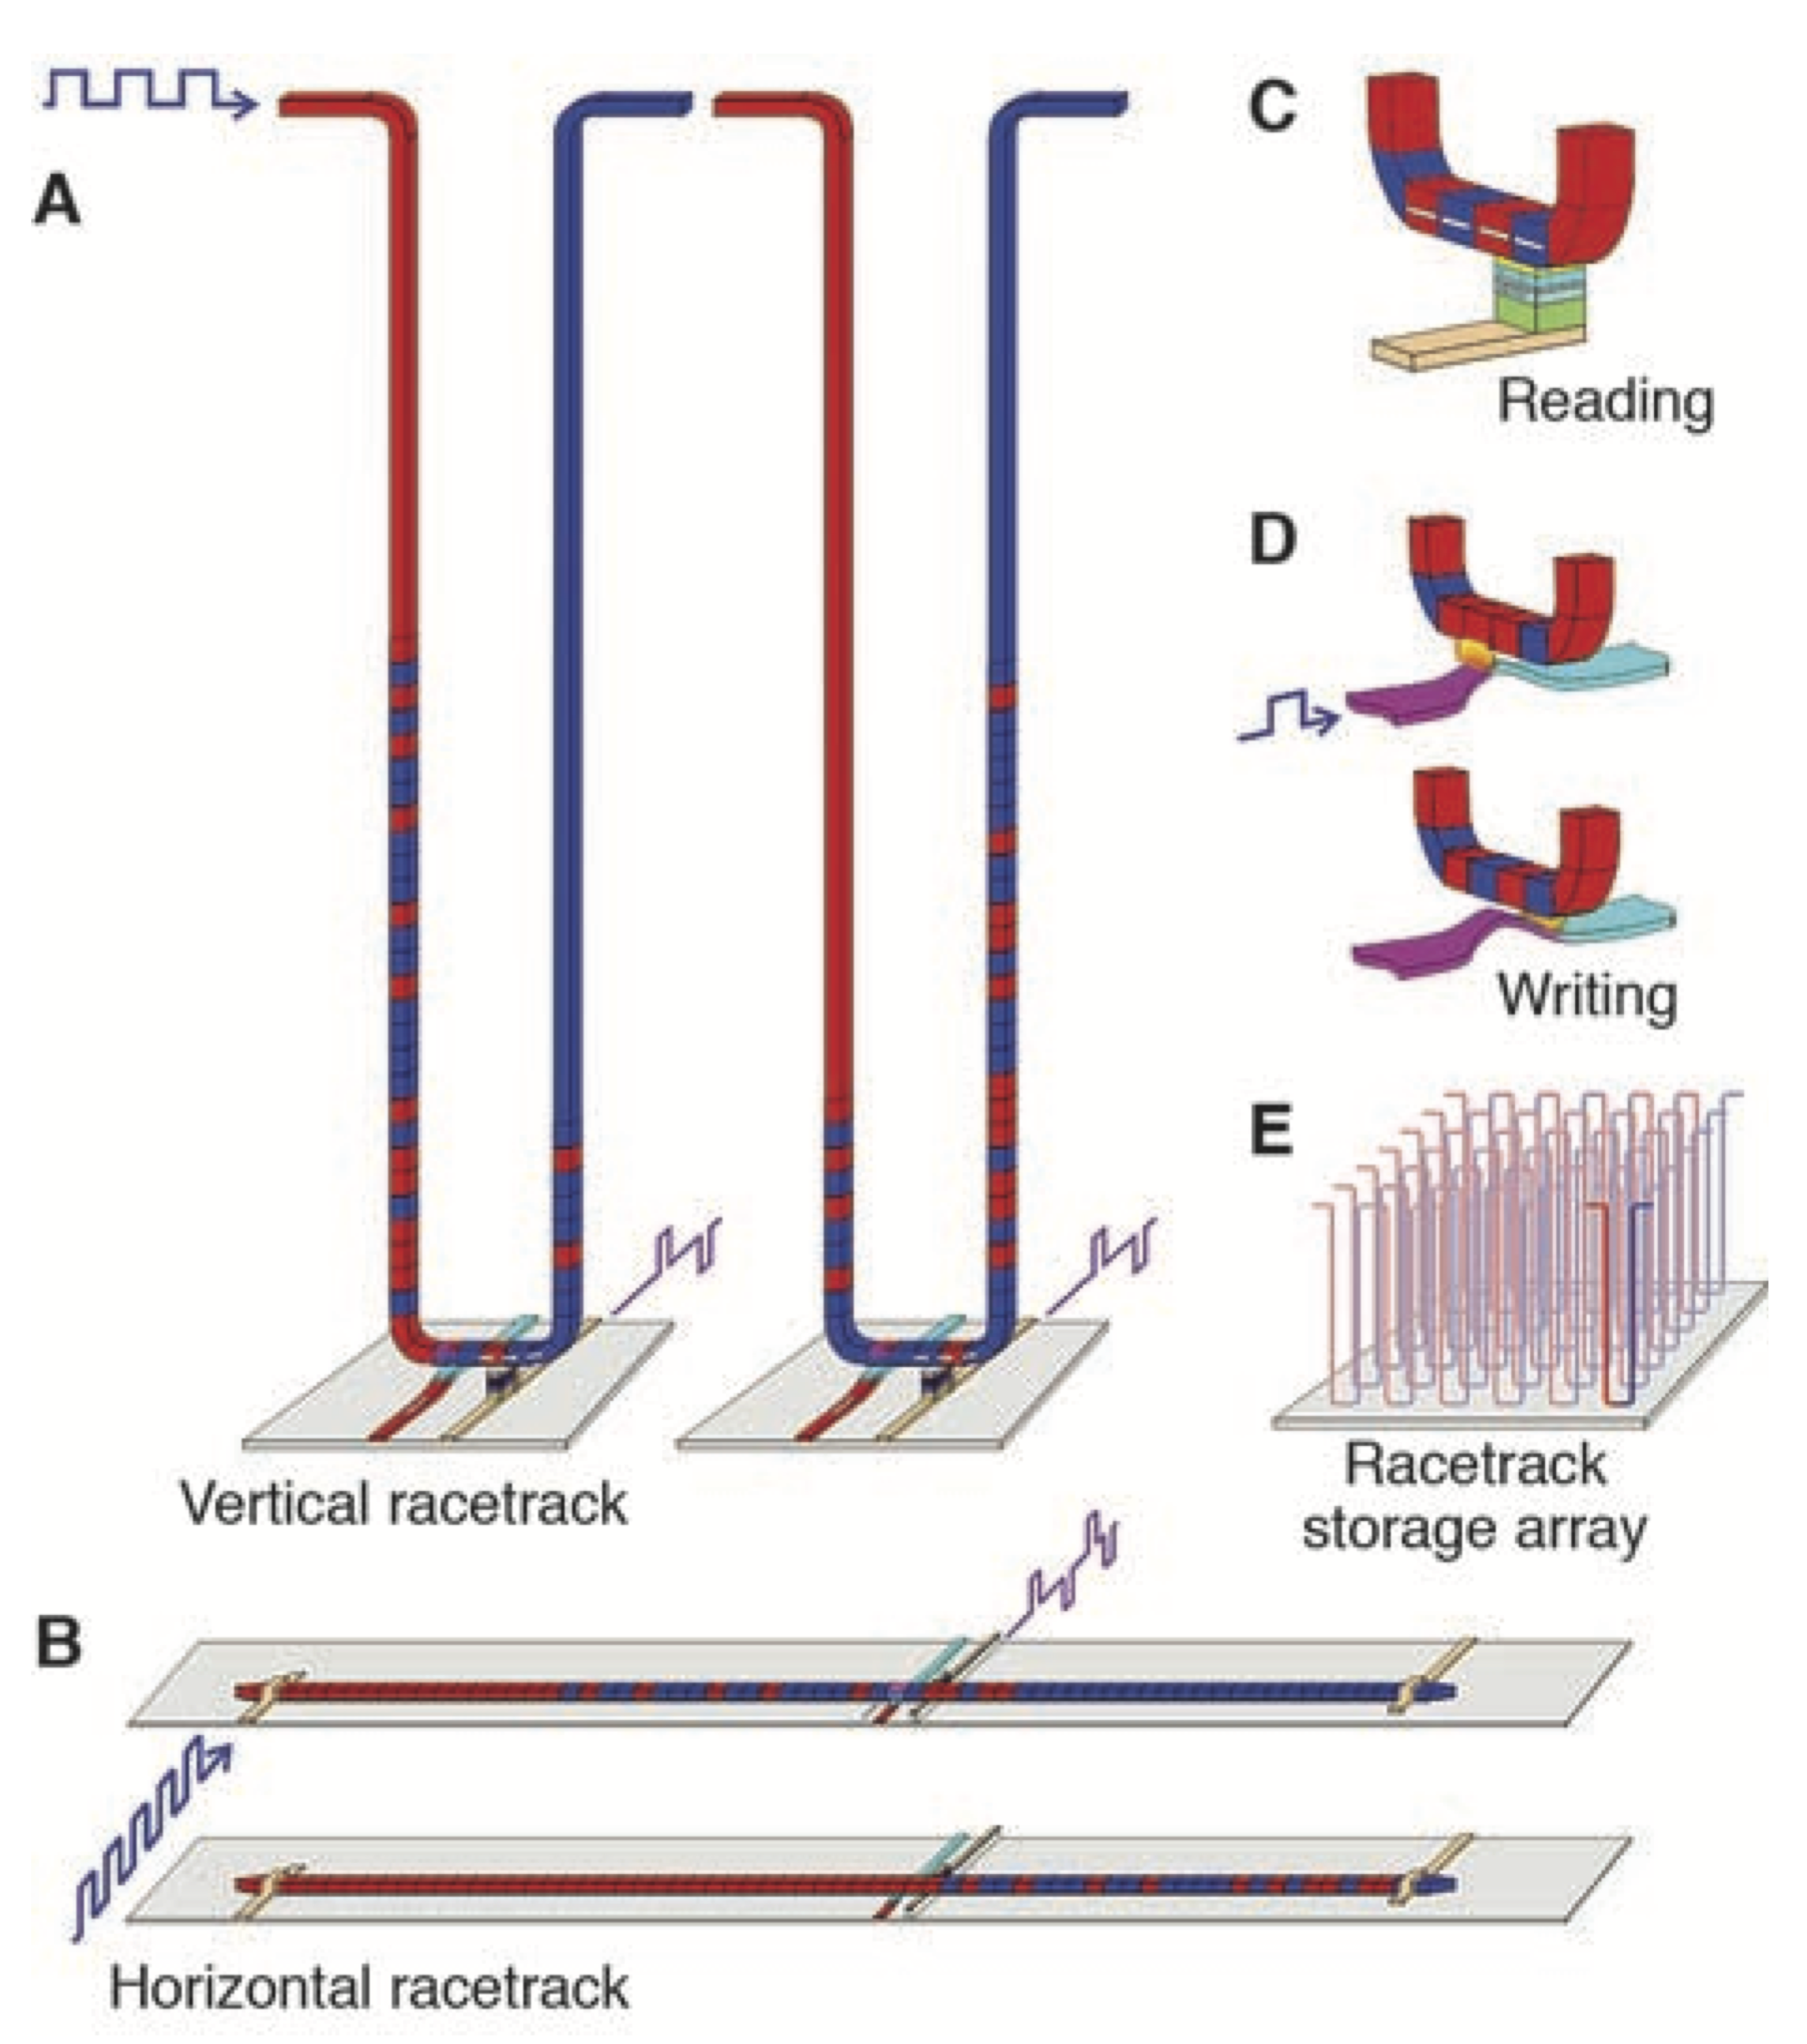
\includegraphics[width=0.9\linewidth]{../figs/RacetrackMemory}
		\end{minipage}				
		\begin{block}{}
		Possible technology for future computer memory
		\end{block}
		
	\end{frame}


			\begin{frame}[c]
		\frametitle{Mathematical Background}
\begin{block}{}
$$
\vec{m}\times\partial_t \vec{m}+\alpha \partial_t \vec{m}+\nabla E_\kappa(\vec{m})(1-\vec{m}\vec{m}^T) = h(1-\vec{m}\vec{m}^T).
$$
\end{block}
		\begin{itemize}
		\item Magnetization $\vec{m}$ a unit vecor
		\item Functional $E_\kappa(\vec{m})$ is the (reduced) internal micromagnetic energy which consists of
the exchange energy from spin interaction, anisotropy energy because of an external magnetic field, and magnetostatic interaction
		\item Traveling wave solutions?
		\item Structure of domain walls?
		\end{itemize}
\begin{center}
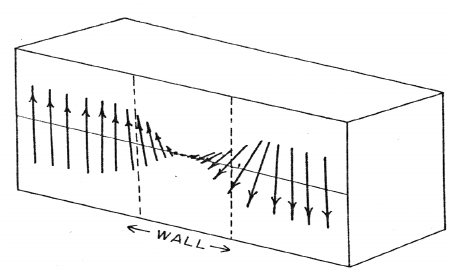
\includegraphics[width=0.4\linewidth]{../figs/BlochWall}
\end{center}
	\end{frame}


	\begin{frame}[c]
		\frametitle{Your Task}
\begin{itemize}
\item Develop numerical tools to study the structure of domain walls (e.g.\ Bloch walls)
\item Develop a simulation model for the dynamics of one-dimensional domain walls
\item Reproduce the theoretical and experimental results from the literature
\item Develop and implement a control strategy to move domain walls by an external magnetic field or by an external current
\end{itemize}				
\begin{center}
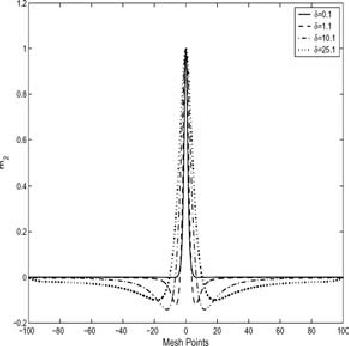
\includegraphics[width=0.3\linewidth]{../figs/Bloch}
\end{center}
	\end{frame}


	
\end{document}
% ---------------------------------------------------------------------------------